 \section{Durchführung}
\label{sec:Durchführung}


\subsection{Aufbau}


\subsubsection{Versuchsaufbau zur Bestimmung des Torsionsmoduls}
\label{sec:AufbauTorsion}

Der Versuchsaufbau besteht aus einem langen Draht, der am oberen Ende an einer
Halterung befestigt ist und an dem am unteren Ende eine Kugel hängt.
An der Halterung ist ein Justierrad angebracht, mit welchem der Winkel
verstellt oder die Schwingung angeregt werden kann.
Die Periodendauer der Schwingung wird mit einer elektronischen Stoppuhr
gemessen. Dabei wird von einer Lampe ein Lichtstrahl auf einen
Spiegel ausgesendet, der am rotierenden System befestigt ist.
Der vom Spiegel reflektierte Lichtstrahl löst bei
bestimmten Auslenkungen den Lichtdetektor aus, sodass ein Signal über eine
digitale Schaltung an die Uhr weitergegeben wird.
Dies ist in Abbildung \ref{fig:AufbauPeriode} abgebildet.
Die Messappatur ohne die Zeitmessvorrichtung ist in Abbildung
\ref{fig:AufbauTorsion} dargestellt.

\begin{figure}
  \centering
  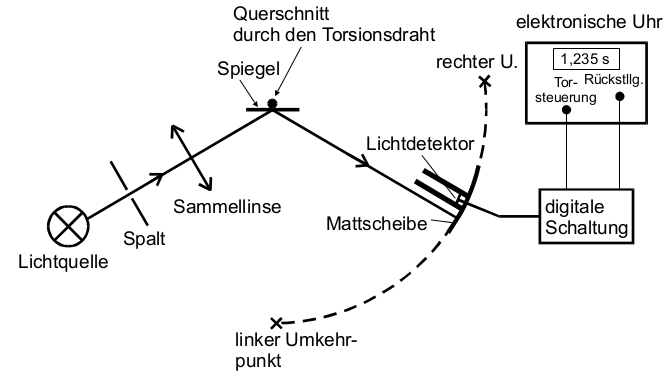
\includegraphics[height=6cm]{Zeitmessung.png}
  \caption{Schematischer Aufbau zur Messung der Periodendauer.}
  \label{fig:AufbauPeriode}
\end{figure}

\begin{figure}
  \centering
  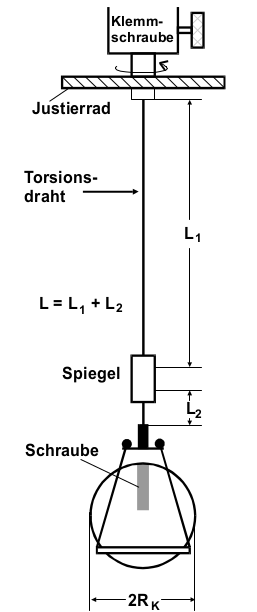
\includegraphics[height=10cm]{ApparaturTorsion.png}
  \caption{Messapparatur zur Bestimmung des Torsionsmoduls.}
  \label{fig:AufbauTorsion}
\end{figure}

\newpage

\subsubsection{Versuchsaufbau zur Bestimmung des magnetischen Momentes }

Der Versuchsaufbau aus \ref{sec:AufbauTorsion} wird um eine Helmholtzspule, die
an eine Konstantstromquelle geschlossen ist, gemäß Abbildung
\ref{fig:AufbauMagnet} erweitert.

\begin{figure}
  \centering
  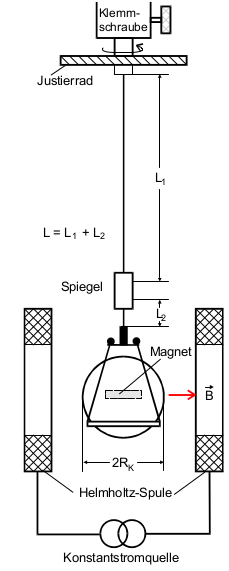
\includegraphics[height=10cm]{ApparaturMagnet.png}
  \caption{Messapparatur zur Bestimmung des magnetischen Momentes.}
  \label{fig:AufbauMagnet}
\end{figure}


\subsubsection{Versuchsaufbau der digitalen Schaltung zur Periodendauermessung}
Abstand!

\subsection{Messprogramm}

\subsubsection{Messprogramm zur Bestimmung des Torsionsmoduls}
\label{sec:MessTorsion}

\begin{itemize}

  \item Zunächst wird die Kugel in die Vorrichtung gelegt, sodass der
  sichtbare Madenschraubenkopf nach oben zeigt. Dann steht der Magnet
  senkrecht zum Erdmagnetfeld, sodass er die Schwingung nicht beeinflusst.

  \item Dann werden Kugel und Draht mit dem Justierrad so rotiert,
  dass der vom Spiegel reflektierte Strahl knapp rechts neben die Photodiode
  fällt. Das System sollte dann in seiner Ruhelage sein.

  \item Als nächstes wird das Justierrad kurz hin und her bewegt, sodass
  das System in einer Rotation zu schwingen beginnt.

  \item Die Messwerte für die Periodendauer werden notiert.

\end{itemize}

\subsubsection{Messprogramm zur Bestimmung des Erdmagnetfeldes}

\begin{itemize}

  \item Durch verstellen des Justierrades wird das System so bewegt,
  dass der Lichtstrahl in der Ruhelage rechts neben die Photodiode fällt.

  \item Die Kugel wird nun so in der Vorrichtung platziert, dass die Schraube
  an der Süd- oder Nordseite zu sehen ist. Dann ist der Magnet parallel zum
  Erdmagnetfeld, sodass die Schwingung davon beeinflusst wird.

  \item Es wird genauso vorgegangen wie in \ref{sec:MessTorsion}.

\end{itemize}

\subsubsection{Messprogramm zur Bestimmung des magnetischen Momentes}

\begin{itemize}

  \item Durch verstellen des Justierrades wird das System so bewegt,
  dass der Lichtstrahl in der Ruhelage rechts neben die Photodiode fällt.

  \item Die Kugel wird nun so in der Vorrichtung platziert, dass die Schraube
  an der Ost- oder Westseite zu sehen ist. Dann sollte der Magnet parallel
  zum Magnetfeld, das durch die Spulen erzeugt wird, und orthogonal zum
  Erdmagnetfeld stehen.

  \item Der Strom wird eingeschaltet und es wird genauso vorgegangen wie in
  \ref{sec:MessTorsion}, wobei darauf geachtet werden muss, dass die Auslenkung
  des Systems gering ist, damit der Einfluss des Magneten über die gesamte
  Periode als maximal angenommen werden kann.

  \item Es werden Messwerte für fünf verschiedene Stromstärken aufgenommen.

\end{itemize}
